% Bhaskar
% fundamental-concepts-fitness-landscapes.tex
%%%%%%%%%%%%%%%%%%%%%%%%%%%%%%%%%%%%%%%%%%%%%%%%%%%%%%%%%%%%%%%%%%%%%%%%%%%%%%%%%%
% revision status as of 2026_03_03
% - [x] accept or reject all track changes
% - [x] incorporate review comments
%    - don’t worry about clearing all comments
% - [x] incorporate reference suggestions
% - [-] cross-cutting revision objectives (see email)
% - [ ] other planned changes or refinements (if any)
% for revision status, mark - for partial or x for complete
% any free-form comments on planned/completed revisions are helpful too!
% --------------------------------------------------------------------------------
% draft status: complete draft as of 2025_11_15
% pick one of: outline, partial draft, rough draft, complete draft
% where rough draft indicates that major points are hit,
% but still working on changes or improvements in refining the text
%%%%%%%%%%%%%%%%%%%%%%%%%%%%%%%%%%%%%%%%%%%%%%%%%%%%%%%%%%%%%%%%%%%%%%%%%%%%%%%%%%


\subsection{Fitness Landscapes}
\label{sec:fitness-landscapes}

% \textbf{Included Citations}: \begin{itemize}
% \item \citet{franke2011evolutionary}
% \item \citet{richter2014fitness}
% \item \citet{reidys2001neutrality}
% \item \citet{eppstein2016quantifying}
% \item\citet{wang2018population}
% \item \citet{dang2016selfadaptation}

% \end{itemize}

% \textbf{Excluded Citations}: \begin{itemize}
% \item \citet{pitzer2012comprehensive}
% \item \citet{reidys2002combinatorial}
% \item \citet{stadler2002fitness}
% \end{itemize}

The \textit{fitness landscape} is a fundamental concept in evolutionary biology that builds upon the idea of a \textit{genotype space}---the space of all possible genetic states that an organism can be in \citep{fragata2019evolution, castle2021towards}. To motivate the general structure of genotype spaces, consider the set of all permutations of a sequence of length $N$, each site in which can contain one of $K$ possible allelic variants. A particular example is the space of $N=3$ bit-sequences where each ``bit" in the sequence can be in $K=2$ states (0 or 1, Fig. \ref{fig:1}). This allows for $K^N$ unique genotypic possibilities. In the case of DNA-based life, $N$ is the size of an organism's DNA sequence (measured in the number of \textit{bases}) and $K$ is the number of possible states of each base in the sequence. In this space, each sequence has $(K-1)N$ \textit{neighbors} that can be obtained by making a single-mutation to the sequence. This number of single-mutation neighbors is referred to as the \textit{dimensionality} of the genotype space, alluding to the number of dimensions required to faithfully capture the linkages and distances in the network. Low dimensional visualization of the genotype space, while instructive, can be misleading \citep{mcleish2015there, greenbury2022structure, gordon1994evolution}. Even in EC, 1- or 2-dimensional solution spaces only occur for 1 and 2 parameter optimization problems. The genotype space is more accurately represented as a network, with the nodes denoting genotypes and edges connecting genotypes that differ by a single mutation (Fig. \ref{fig:1}, left).

\begin{figure}
    \centering
    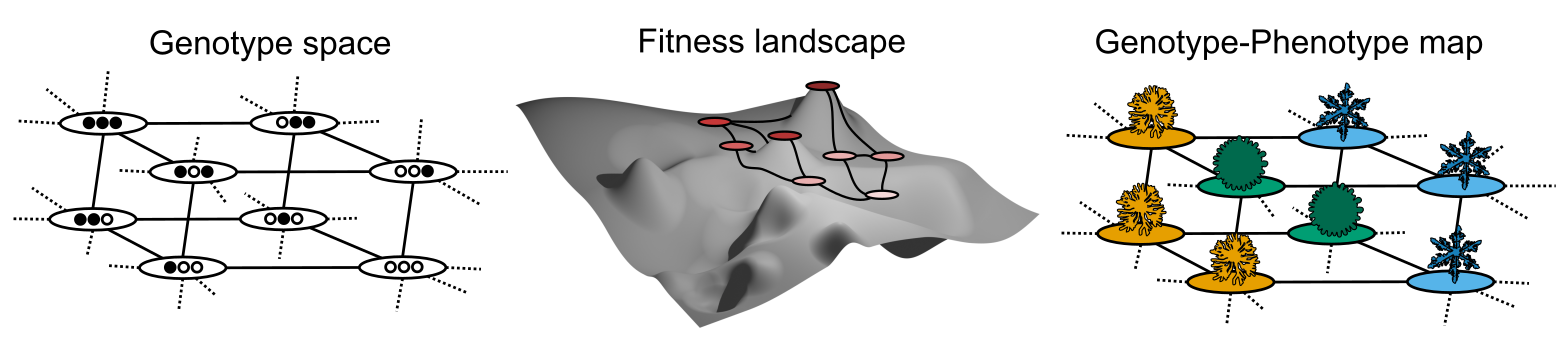
\includegraphics[width=1.0\linewidth]{img/fitness_landscapes.png}
    \caption{\textbf{Three flavors of biological genetic spaces}. The \textit{genotype space} (left) is a network of genotypes, with edges connecting genotypes that differ by a single mutation. A subset of a much larger genotype space is shown here, consisting of two alternative allelic states ($K=2$, filled or open circle) at three sites ($N=3$). A \textit{fitness landscape} (middle) is induced on this space when each genotype is assigned a value denoting its reproductive success in an environment. One may draw this landscape with the fitness values along a third dimension. However, this visualization only works for 2-dimensional genotype spaces, which are rare (if not absent) in biological systems. Even the simple genotype space shown here cannot be drawn as a planar network. Alternatively, the genotypes may be assigned ``phenotypes'' that denote the visible characteristics of the resulting organisms (e.g. colony morphology of a bacterium). This mapping of genotypes to phenotypes on an existing genotype-space forms the \textit{genotype-phenotype map} (right).}
    \label{fig:1}
\end{figure}

A fitness landscape is induced when each node in the genotype space is mapped to a fitness value in a given environment (Fig. \ref{fig:1}, middle). The fitness landscape thus captures not only the mapping between genotype and fitness, but also the spatial correlation between these fitness values in the genotype space. In EC, the search space plays an equivalent role by linking possible solutions of a problem to the value of an objective function that is to be optimized \citep{back1996evolutionary, foster2001evolutionary, richter2014fitness}. Due to the spatial nature of this mapping, topographic metaphors like ``peaks'' and ``valleys'' have become extremely popular in evolutionary biology as they convey structural information about the fitness landscape in a manner that is easily visualized \cite{martin2013multiple, steinberg2016environmental}. ``Peaks" denote genotypes that are locally fitter than their immediate mutants, while ``valleys" denote genotypes that are locally deleterious compared to their mutants in terms of fitness. Biological fitness landscapes tend to have many such peaks and valleys, making them incredibly \textit{rugged} \citep{papkou2023rugged, reidys2001neutrality}. This ruggedness makes it difficult for adaptive evolution to explore the genotype space exhaustively, as populations may get stuck on locally optimal peaks \citep{li2025probability, bank2022epistasis, neidhart2014adaptation}. A similar problem arises in EC, where a solution space with many local optima prevents algorithms from converging to globally optimal solutions. Stochastic algorithms that can move vast distances in the genotype space in a few steps are sometimes necessary to sample the solution space somewhat exhaustively \citep{fogel1994introduction, fouskakis2002stochastic}. The use of \textit{recombination} or \textit{crossover}, a technique that combines different promising solutions in order to generate a new hybrid candidate can also allow such jumps in the genotype space in a way that is biased towards functional sequences/solutions, and is an important process in both biological evolution and evolutionary computation \citep{li2024rapid, doerr2008crossover, fogel1994effectiveness}.

%Criticism of the metaphor
While extremely useful in certain situations, the fitness landscape metaphor has drawn criticism for multiple reasons \citep{gavrilets1997evolution}. As described earlier, the low-dimensional picture used to convey this idea, while helpful, is not the most accurate. Further problem arises when this visualization is used to explain phenomena that proceed on spaces with very high dimensionality, where the  intuition that is useful in 2 or 3 dimensions breaks down. Larger dimensionality can have wide-ranging effects on evolutionary dynamics.  For example, even though the spaces are complex, most genotypes can be accessed \textit{adaptively} through only a few mutational steps, especially in spaces with a high dimensionality \citep{franke2011evolutionary}. Subsequently, it is possible to find global optima relatively easily on biological landscapes as the dimensionality of the genotype space increases. Further, the fitness landscape picture imagines a static mapping between genotype and fitness. This is not generally true as changes in the population composition may change the landscape due to density dependent effects \citep{kaplan2008end}. Thus, a fixed landscape does not capture the dynamic nature of fitness in most living systems. In light of this, alternative formulations like the "fitness seascape" have been proposed \citep{cairns2022strong, mustonen2009fitness}. A faithful picture of the biological solution space would require the ability to visualize networks in multiple dimensions, one which we currently lack. Like many other intuition building analogies in the sciences, the idea of fitness landscape is limited in its ability to allow predictions of the fate of evolving populations \citep{achinstein1964models}.

The \textit{genotype-phenotype} map (\textit{GP-map}) is an alternate formulation of the fitness landscape idea that maps genotypes to discrete, visible traits of an organism (the \textit{phenotype}) and thus separates the relationship into three distinct layers \citep{ahnert2017structural, aguilar2018architecture}. This intermediate phenotype layer decouples the environment dependent genotype-fitness relationship into a relatively invariant genotype-phenotype map and a phenotype-fitness map that may change with the environment. In biological systems, phenotypes arising from a genotype might themselves be environment dependent---for example, a developmental gene may be expressed differently depending on the temperature. Such environmental dependencies are rarely encountered in EC because the ``phenotypes", if they exist, are evaluated well before the candidate solution is exposed to the problem \citep{moczek2011role}. Some fields of EC like deep learning, however, do rely on direct environmental input to determine the phenotype and subsequently the fitness of a solution  \citep{zhan2022evolutionary}.  Like the fitness landscape, the structure of the genotype-phenotype map has also been of great interest in evolutionary biology, partly because phenotypes are easier to measure than fitness and partly due to the relatively stable nature of the mapping under environmental change \citep{chen2022environmental, ahnert2017structural, wagner2011pleiotropic, aguilar2018architecture}

The structure of the genotype-phenotype map can be equally instructive as fitness landscapes in understanding how evolutionary dynamics operate on genotype spaces. Phenotypically contiguous parts of the GP-map are sometimes referred to as \textit{neutral networks} as they allow populations to acquire mutations ``neutrally", without any effect on phenotypes or fitness \citep{reidys2001neutrality, ahnert2017structural, croitoru2022punctuated}. Such neutral networks have been shown to promote \textit{mutational robustness} as a genotype within a neutral network can acquire many successive mutations without any apparent effect on fitness \citep{van1999neutral}. Additionally, large neutral networks can allow populations to drift across the genotype space without a fitness cost, thus promoting evolutionary innovations in the long-term \citep{jorg2008neutral, huynen1996smoothness, shackleton2000investigation, huynen1996exploring, amitai2007latent, banzhaf2006evolution, hu2025neutrality}.  This process has been used to resolve a long debate on tradeoffs between robustness and evolvability in such genotype spaces---mutational robustness may inhibit evolutionary innovation on short time scales but can promote it over the long term \citep{wagner2008robustness, wagner2013robustness, masel2010robustness, hu2018neutrality}. Work on empirical fitness landscapes has also shown the presence of many \textit{evolvability-enhancing} mutations in biological fitness landscapes that enable further adaptive evolution while not necessarily being equivalently adaptive themselves \citep{wagner2023evolvability}.

The GP-map  and the induced fitness landscape also allow us to study how local structures in the genotype space can aid populations during evolution. Boundaries between phenotypes on the GP-map can act as hot-spots that aid evolutionary rescue in response to environmental change \citep{kumawat2025evolution, ancel2005evolution, kussell2006polymerpopulation}. The set of phenotypes accessible through mutations on these boundaries can even encode measurable information about the various environments encountered during evolution \citep{kumawat2025evolution}. Further, the structure of the fitness landscape may limit the effectiveness of evolutionary control methods used to suppress the growth of harmful microbial populations or for directed evolution. For example, researchers have shown that abundant edge-flips in a fitness landscape--i.e, single mutation edges that change the direction of adaption between two mutants in two environments, can allow us to predict the efficacy of intermittent antimicrobial therapy \citep{chen2024inverted}. Similarly, a measure called the mutation effect reaction norm (Mu-RN) has been used to quantify the effect of mutations across environments \citep{ogbunugafor2022mutation}. Work on drug resistant mutations has also formalized the idea of \textit{deception} on fitness landscapes, which is the presence of epispastic mutations that lead populations away from global optima \citep{eppstein2016quantifying, ogbunugafor2016competition}. Biological literature thus provides an abundance of structural properties that can be directly translated into the EC domain to motivate the design of solution spaces and algorithms that leverage second-order outcomes of the evolutionary process. 

One of the major takeaways from the work on fitness landscapes is that the solution space, in biology and in EC, can rarely be explored in an unconstrained manner---i.e., new candidate solutions only arise from old ones, and thus the underlying \textit{representation} of the solution space controls the malleability of the genome after mutations, which in-turn translates to variations in fitness for a given objective \citep{ashlock2012representation}. New algorithms may be selected for a given problem based on metaheuristic analyses that try to take these representations into account \citep{wang2018population}.  On-line optimization of parameters during evolutionary searches is also a promising area of study when trying to overcome the limits of a given representation \citep{dang2016selfadaptation}. In many cases, the fitness landscape structure also changes based on the environment that a population experiences. In evolutionary biology, the term ``fitness seascape" has been used to describe a set of fitness landscapes with the same underlying genotype space but various fitness values spanning multiple environments \citep{mustonen2009fitness}. In the context of EC, such fitness seascapes may appear when either the nature of the optimization problem is changed or if new training data is introduced, for example in the case of online learning. Seascapes can also be used to describe the changing effective fitness landscapes in cases where a diversity maintenance mechanism is implemented to increase exploration of the solution space, or when adversarial algorithms evolve together with the main solution \cite{dolson2021digital}. The role of such changing fitness landscapes, or seascapes, in EC optimization problems remains insufficiently explored \citep{grefenstette1999evolvability, richter2009detecting}.
